\documentclass[onecolumn]{article}
\usepackage{graphicx}
\usepackage{float}
\usepackage{listings}
\lstset{language=Fortran}
\restylefloat{figure}
\begin{document}

\title{Using coarrays to solve a domain-decomposition problem}

\author{Arjen Markus}

\maketitle

\section{Introduction}
Coarrays have been part of the Fortran standard since the 2008 standard, but their use does not seem to be ubiquitous.
See \cite{ModernFortran2023} for a description of this feature. This note tries to demonstrate that designing a parallel algorithm
that uses coarrays can be straightforward, although, as usual with parallel programs, it is not always easy. The algorithm
in question concerns the solution of a diffusion equation on a rectangular grid. To enhance the performance, the grid is
split up into smaller rectangular areas, subgrids or \emph{domains}, each of which is assigned to a single \emph{image}.\footnote{The program described here is based on a
regular two-dimensional rectangular grid, but that is for the sake of simplicity only. We want to focus on the coarray aspects in a non-trivial situation.}
The complication is that each subgrid needs to communicate with its neighbours and that is where the coarray feature comes in.

The methodology is demonstrated with a small program. The numerical method used is the simplest possible, so that all emphasis
is on the coarray aspects. The concentration in grid  cell (i,j) is calculated via the following explicit formula:
\begin{eqnarray}
    C_{i,j}^{t+ \Delta t} &=& C_{i,j}^t  + \frac{ D \Delta t}{\Delta x^2} \bigl( C_{i-1,j}^t + C_{i+1,j}^t + C_{i,j-1}^t + C_{i,j+1}^t - 4 C_{i,j}^t \bigr)
\end{eqnarray}

\noindent where the combination $D \Delta t / \Delta x^2$ can be abbreviated to a single factor, as the explicit factors do
not play an independent role (see the description of the input).

\begin{figure}[H]
\caption{Sketch of the subgrid. The grid cells in gray are the boundary cells. The grid dimensions are 3 rows and 4 columns
-- the boundary cells are added to this.}
\label{subgrid}
\begin{center}
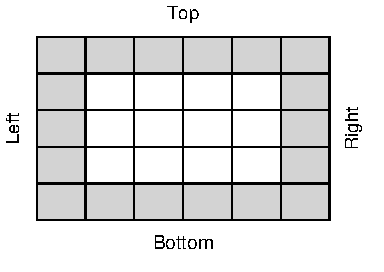
\includegraphics[width=0.9\textwidth]{diagram_subgrid.pdf}
\end{center}
\end{figure}


\section{The grid layout}
A sketch of a subgrid, with some terminology, is shown in Figure \ref{subgrid}. The four sides of the grids are
represented by an extra row or column of grid cells, so that the boundary conditions can be taken care of. There are
three types of boundary condition in the program:
\begin{itemize}
\item
The concentration on the boundary can have a fixed value -- constant in time and along the boundary.
This is implemented by setting the concentration in the extra grid cells to that value at the start of the calculation.
\item
The diffusive flux over the boundary is zero -- mathematically speaking, $\partial C / \partial \underline{n} = 0$
This can be implemented effectively by copying the concentration in the row or column of grid cells next to the boundary cells
into these boundary cells at each time step. The discretised flux is then zero.
\item
The side is adjacent to that of another subgrid. Then the concentrations on the inside of both subgrids will have to be copied
to the adjacent subgrid -- see picture \ref{adjacent}. Again, this has to happen at each time step, or at least frequently enough.
\end{itemize}

Thus, the boundary conditions are simple enough to allow the \emph{same} formula to be used for all internal cells:
\begin{lstlisting}
    dconc = 0.0
    dconc(2:length+1,2:width+1) = &
        diff_factor * ( conc(1:length,2:width+1) &
                        + conc(3:length+2,2:width+1) &
                        + conc(2:length+1,1:width) &
                        + conc(2:length+1,3:width+2) &
                       - 4.0 * conc(2:length+1,2:width+1) )
    conc  = conc + dconc
\end{lstlisting}

This can be made slightly more compact by calculating the new concentration directly, instead of via an array for the
derivative. However, the derivative can easily be used in a further refinement of the program to determine if convergence has been reached yet.

\begin{figure}[H]
\caption{Boundary condition for two adjacent subgrids. The concentration in the orange cells on the left is copied to the boundary cells on the right.
Similarly for the lightblue cells, but then from right to left.}
\label{adjacent}
\begin{center}
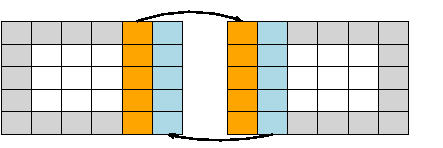
\includegraphics[width=0.9\textwidth]{diagram_adjacent.pdf}
\end{center}
\end{figure}


\section{The demonstration program}
To make the demonstration a bit more interesting, the program uses a fairly flexible method to construct the complete grid:\footnote{The program is listed in the appendix for easy reference.}
\begin{itemize}
\item
Each subgrid is defined in an input file of its own. The definition should include the dimensions (number of rows and columns, without the extra rows and
columns for the boundaries), the types of boundaries and either the value to be applied or the subgrid to which it is adjacent.
\item
The first subgrid may contain the number of time steps to calculate and the diffusion parameter, a combination of the actual time step, the diffusion
coefficient and the grid cell size (assumed to be the same in both x and y directions).
\end{itemize}

For example:

\begin{verbatim}
# Corner: lower-left
#
grid 20 20
left-boundary open 1.0
right-boundary image 2
top-boundary closed
bottom-boundary closed
initial 1.0

timespan 1000
diff-factor 0.1
\end{verbatim}

The demonstration program uses three subgrids that are arranged as shown in Figure \ref{domains}.

\begin{figure}[H]
\caption{Domains in the sample calculation.}
\label{domains}
\begin{center}
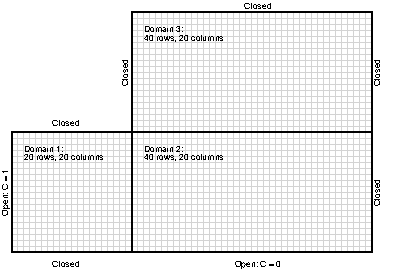
\includegraphics[width=0.9\textwidth]{diagram_domains.pdf}
\end{center}
\end{figure}

The input is read by a separate subroutine, \verb+read_input+, which fills a data structure \verb+domain+ with the information that is specific
for the subgrid. Since the variable is a \emph{local} variable, each image has its own variable, independent of the other images.

Two complications occur:
\begin{itemize}
\item
As we define the complete grid via fixed subgrids, we may have more images than there are subgrids. That means a number of subgrids will be
idle. In the program we deal with this situation by distinguishing two so-called \emph{teams}, images that act as a separate group and can be
synchronised independently of the other groups:

\begin{lstlisting}
    write( filename, '(a,i0,a)' ) 'corner_', this_image(), '.inp'

    open( 10, file = filename, status = 'old', iostat = ierr )

    if ( ierr == 0 ) then
        running_image = this_image()
        call read_input( domain )

        write(*,*) 'Image ', this_image(), domain, ' --> ', running_image
        this_team = 1
    else
        this_team = 2
        write(*,*) 'Image ', this_image(), ' inactive'
    endif

    !
    ! We need to make sure all images have finished the initialisation
    !
    form team ( this_team, active_inactive )
\end{lstlisting}

Almost the whole program is now split into two parts via the \verb+change team+ construct:
\begin{lstlisting}
    !
    ! Select the team and enter the team construct
    !
    change team ( active_inactive )

        if ( team_number() == 1 ) then
            ... Actual calculation
        else
            !
            ! The second team has no task ...
            !
            write(*,*) 'Image ', this_image(), ' is idle'
        endif
    end team
\end{lstlisting}

\item
We need to give the arrays that are used to exchange the boundary values, \verb+left_concentration+ etc., a size that is first of all equal on
each image (a requirement for coarrays) and that is large enough to fit all sides in the whole grid that are shared by two subgrids. In the
figure domain 1 is adjacent to domain 2, and domain 2 is also adjacent to domain 3. The longest shared side in the horizontal direction therefore
covers 40 (plus 2) grid cells and the longest shared side in the vertical direction covers 20 (plus 2) grid cells.

The collective coarray routine \verb+co_max+ comes in very handy. The \emph{local} variables \verb+xmax+ and \verb+ymax+ are first set to the
domain size in each image and then set via this routine to the maximum over all images:

\begin{lstlisting}
    !
    ! Prepare the calculation
    !
    xmax = domain%nx
    ymax = domain%ny
    call co_max( xmax )
    call co_max( ymax )
\end{lstlisting}

The maximum value is broadcast to all images, so that they can allocate the coarrays for the boundaries:

\begin{lstlisting}
    allocate( left_concentration(ymax+2)[*]   )
    allocate( right_concentration(ymax+2)[*]  )
    allocate( top_concentration(xmax+2)[*]    )
    allocate( bottom_concentration(xmax+2)[*] )
\end{lstlisting}

We can use the codimension \verb+[*]+, because the subgrids have no particular ordering. In more complex situations you may want to
arrange the images in some grid of their own and then a multi-dimensional codimension is useful \cite{CellularAutomataCoarrays}.

The concentration array and the array with the time derivative are local arrays that should be allocated to the size of the subgrid
that is associated with the image, very classically:

\begin{lstlisting}
    allocate( conc(domain%nx+2,domain%ny+2)  )
    allocate( dconc(domain%nx+2,domain%ny+2) )
\end{lstlisting}

\emph{Note:} the concentration array might be made a coarray too, for easier collecting the information over the whole grid for output.
In this program the end result per subgrid is written to a separate file instead. A postprocessing program could then stitch the
results together for presentation purposes.
\end{itemize}

\subsection{Computational core}
The heart of the program is the loop over time where the new concentration is calculated and the boundary conditions are exchanged.
An excerpt is shown below:

\begin{lstlisting}
   !
   ! Do the calculation
   !
   do i = 1,timespan

       dconc = 0.0
       dconc(2:length+1,2:width+1) = diff_factor * ( ... )

       conc  = conc + dconc

       left_concentration(1:width+2)    = conc(2,:)
       right_concentration(1:width+2)   = conc(length+1,:)
       top_concentration(1:length+2)    = conc(:,width+1)
       bottom_concentration(1:length+2) = conc(:,2)

       !
       ! Wait for all the images before copying the boundaries
       ! (note: sync all works on the current team, which is not the initial team at this point)
       !
       sync all

       ! Left
       if ( domain%boundary_type(1) == 2 ) then
           conc(1,:) = right_concentration(1:width+2)[domain%connecting_domain(1)]
       elseif ( domain%boundary_type(1) == 0 ) then
           conc(1,:) = conc(2,:)
       endif

       !
       ! Similarly the other sides
       !
       ...

       !
       ! And when everything has been copied, continue
       !
       sync all
   enddo
\end{lstlisting}

There are two instances of the \verb+sync all+ statement: the first to make sure all images within the team are ready with the current
time step and also have filled the array to exchange the boundary data and the second to actually exchange the boundary data and
make sure all are ready for the next step.\footnote{The \emph{sync all} statement only synchronises the images in the current team, not all images.}
The fragment in between the two statements uses the coarrays to do the exchange.


\section{Summary}
A summary of the demonstration program may be useful:
\begin{itemize}
\item
The first step is to read the input files that define the domains (subgrids). Each domain is associated with one image.
\item
To manage the images that are \emph{not} associated with a domain, two teams are formed. The second team simply waits for the calculation
to finish.
\item
The first team, however, does the integration over time and exchanges the boundary data at each time step. For this synchronisation is
required, otherwise we cannot be sure that the data that are copied from one domain to the other are consistent.
\item
When the calculation has finished, the resulting concentrations are written to separate files, so that they can be visualised (see Figure \ref{domains}). This is
simply an easy solution, probably not the best possible.
\end{itemize}

\begin{figure}[H]
\caption{Solution of the diffusion problem on three domains in an L-shape. (Courtesy Ivan Pribec.)}
\label{domains}
\begin{center}
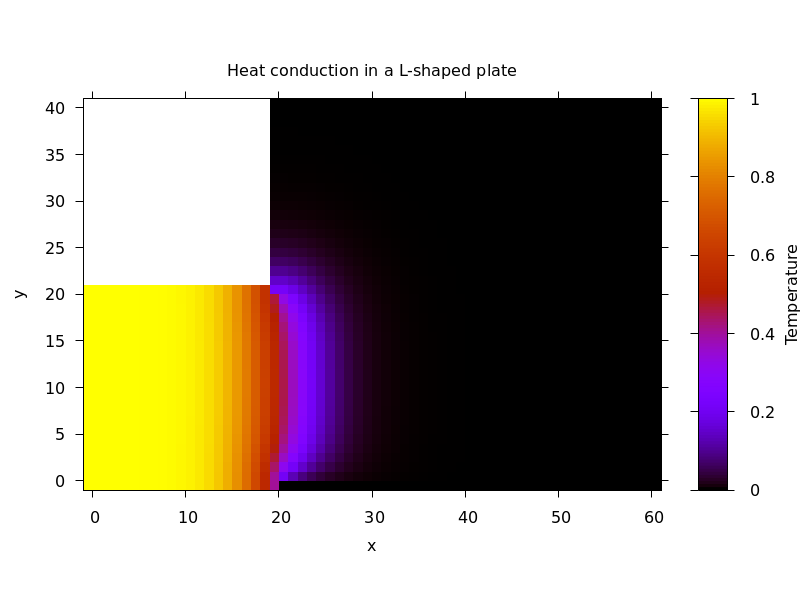
\includegraphics[width=0.9\textwidth]{report_corner.png}
\end{center}
\end{figure}


\section{Caveats}
The program was written in several stages -- the description above is the end result. The earlier stages are, however, also of interest and
they are described in some detail in this section.

Some emphasis has been put on the management of the inactive images. This is, because they are waited upon by the \verb+sync all+ statements.
If they are stopped early in the program's execution, such as after noticing that they are not associated to a domain:
\begin{lstlisting}
    open( 10, file = filename, status = 'old', iostat = ierr )

    if ( ierr == 0 ) then
        running_image = this_image()
        call read_input( domain )

        write(*,*) 'Image ', this_image(), domain, ' --> ', running_image
    else
        write(*,*) 'Image ', this_image(), ' stopped'
        stop
    endif
\end{lstlisting}
\noindent the \verb+sync all+ statements will wait forever.

Attempts to use the \verb+sync images+ statement instead and only wait for the active images failed for unknown reasons. The program would
simply lock up in the same way as with \verb+sync all+.

The alternative was to detect that some images were inactive and then stop the program: the user would have to set the environment variable
that controls the number of images, \verb+FOR_COARRAY_NUM_IMAGES+ for the Intel Fortran compiler, or specify the default number of images at
compile time. As this is a somewhat unfriendly method, the final version uses teams. And as can be seen in the code, that is rather easy
to accomplish in this case.


\section{An MPI-based equivalent}
With this coarrays-based version completed, it became obvious that an MPI-based version should follow. The demonstration program
does not require much complicated interaction, so it should be easy to transform it to use MPI instead. Just as with the
coarrays, each process, the MPI equivalent of "image", takes care of one subgrid. But there were some tricky parts:

\begin{itemize}
\item
While in the coarrays version an image addresses the arrays on the neighbouring images directly, this is not possible with MPI: there you
send a message to the receiving process which is the neighbour in the multidomain set-up,
and this should actively pick it up. So there is more explicit cooperation required.
\item
Each process needs to know which subgrids are adjacent. One solution would be for each process to send messages to each
other process to relay this information, but with $N$ subgrids, this would mean $4(N-1)$ messages per subgrid, or roughly $4N^2$ in total.
If $N$ is small, this is not a real problem, but suppose you have 100 or 1000 subgrids, then this might become a serious matter.
In a two-dimensional geometry, you would expect only in the order of $4N$ interfaces.
\item
You need to make sure that the processes have received the messages and have processed the information. There is probably
a clear construction to achieve this, but it seemed cumbersome. Instead, the solution chosen here was to have the main process
gather the information from each subgrid on its neighbours and then send that
entire piece of information to each process, so that it could determine what subgrids are adjacent.
\end{itemize}

All in all, the following fragment implements this information exchange:

\begin{lstlisting}
    call MPI_GATHER( domain%connecting_domain, size(domain%connecting_domain), &
                     MPI_INTEGER, connection, size(connection,1), &
                     MPI_INTEGER, root, MPI_COMM_WORLD, ierror )

    call MPI_Barrier( MPI_COMM_WORLD, ierror )

    call MPI_BCAST( connection, size(connection), MPI_INTEGER, root, &
                    MPI_COMM_WORLD, ierror )

    call MPI_Barrier( MPI_COMM_WORLD, ierror )

    do j = 1,size(connection,2)
        do i = 1,size(connection,1)
            if ( connection(i,j) == process_Rank+1 ) then
                domain%destination(side(i)) = j - 1      ! Shift by 1 required
            endif
        enddo
    enddo
\end{lstlisting}

Now each process has all the information necessary: it knows which of its sides are adjacent to which
subgrid (or whether it is simply an external boundary).

Sending the results of time $T$ to the correct neighbour requires a message for this neighbour:

\begin{lstlisting}
    if ( domain%destination(1) /= -1 ) then
        call MPI_SEND( left_concentration,   width+2,  MPI_REAL, &
                       domain%destination(1), 2, MPI_COMM_WORLD, ierror )
    endif
\end{lstlisting}

(Note: the literal \verb+2+ is the encoding of the right-hand side of the neighbour. A symbolic name -- parameter -- would have been better.)

The neighbour should in turn pick up the message:

\begin{lstlisting}
    if ( domain%boundary_type(2) == 2 ) then
        call MPI_RECV( left_concentration, width+2, MPI_REAL, &
                       domain%connecting_domain(2)-1, 2, &
                       MPI_COMM_WORLD, status, ierror )
        conc(length+2,:) = left_concentration(1:width+2)
    elseif ( domain%boundary_type(2) == 0 ) then
        conc(length+2,:) = conc(length+1,:)
    endif
\end{lstlisting}

The program that resulted probably contains too much "juggling" of the IDs of the various subgrids. This is partly due to the fact that with MPI
the process IDs start with zero instead of one, as with coarrays, and I wanted the code to stay as close to the coarrays version as
possible. Another reason is that the left-hand side in one subgrid is the right-hand side in the adjacent subgrid. This may have confused
the coding more than necessary. But whatever the merits and shortcomings of this second demo program, it does work and gives exactly
the same results as the coarrays version.


\appendix
\section{Source code of the coarrays version}
The source of the demonstration program is shown here in full. It contains traces of its development, such as extra output to see what is happening.
It could also be useful to characterise the sides by integer parameters instead of the literal numbers 1, 2, 3 and 4.

Also note: There is no guarantee that the program is flawless. (The listing is shown in a fixed-size font, because of the page width.)

\begin{small}
\begin{verbatim}
! corner.f90 --
!     Solve a diffusion problem defined on several connected domains
!
!     Note:
!     Stopping the images that have no role in the calculation means
!     that a "sync all" statement causes a deadlock. It will wait for
!     all original images.
!
!     Hm, keeping a list of running images does not solve the problem
!     At least not with this version of Ifort (2021.9.0)
!
!     Use teams to split off the inactive images
!
program corner
    use iso_fortran_env

    implicit none

    type(team_type) :: active_inactive

    type domain_type
        integer               :: nx, ny
        integer, dimension(4) :: boundary_type          = -1
        integer, dimension(4) :: connecting_domain      = -1
        real, dimension(4)    :: boundary_value         = -999.0
        real                  :: initial_concentration  = -999.0
    end type domain_type

    type(domain_type) :: domain

    real, allocatable :: left_concentration(:)[:]
    real, allocatable :: right_concentration(:)[:]
    real, allocatable :: top_concentration(:)[:]
    real, allocatable :: bottom_concentration(:)[:]
    real, allocatable :: conc(:,:)
    real, allocatable :: dconc(:,:)

    integer, allocatable :: running_image[:]
    integer, allocatable :: list_running_images(:)

    character(len=80) :: filename
    integer           :: i, ierr
    integer           :: xmax, ymax, length, width
    integer           :: this_team

    integer           :: timespan
    real              :: diff_factor

    allocate( running_image[*] )
    running_image = 0

    write( filename, '(a,i0,a)' ) 'corner_', this_image(), '.inp'

    open( 10, file = filename, status = 'old', iostat = ierr )

    if ( ierr == 0 ) then
        running_image = this_image()
        call read_input( domain )

        write(*,*) 'Image ', this_image(), domain, ' --> ', running_image
        this_team = 1
    else
        this_team = 2
        write(*,*) 'Image ', this_image(), ' inactive'
    endif

    !
    ! We need to make sure all images have finished the initialisation
    !
    form team ( this_team, active_inactive )

    !
    ! Select the team and enter the team construct
    !
    change team ( active_inactive )

        if ( team_number() == 1 ) then

            !
            ! Prepare the calculation
            !
            xmax = domain%nx
            ymax = domain%ny
            call co_max( xmax )
            call co_max( ymax )

            call co_broadcast( timespan, 1 )
            call co_broadcast( diff_factor, 1 )

            if ( this_image() == 1 ) then
                write(*,*) 'Overall grid sizes: ', xmax, ymax
            endif

            allocate( left_concentration(ymax+2)[*]   )
            allocate( right_concentration(ymax+2)[*]  )
            allocate( top_concentration(xmax+2)[*]    )
            allocate( bottom_concentration(xmax+2)[*] )

            allocate( conc(domain%nx+2,domain%ny+2)  )
            allocate( dconc(domain%nx+2,domain%ny+2) )

            !
            ! Set up the concentrations
            !
            length = domain%nx
            width  = domain%ny

            if ( domain%initial_concentration /= -999.0 ) then
                conc = domain%initial_concentration
            else
                conc = 0.0
            endif

            ! Left
            if ( domain%boundary_type(1) == 1 ) then
                conc(1,:) = domain%boundary_value(1)
            endif
            ! Right
            if ( domain%boundary_type(2) == 1 ) then
                conc(length+2,:) = domain%boundary_value(2)
            endif
            ! Top
            if ( domain%boundary_type(3) == 1 ) then
                conc(:,width+2) = domain%boundary_value(3)
            endif
            ! Bottom
            if ( domain%boundary_type(4) == 1 ) then
                conc(:,1) = domain%boundary_value(4)
            endif

            !
            ! Do the calculation
            !
            do i = 1,timespan
                if ( mod(i,100) == 0 ) then
                    write(*,*) this_image(), i
                endif

                dconc = 0.0
                dconc(2:length+1,2:width+1) = &
                    diff_factor * ( conc(1:length,2:width+1) + conc(3:length+2,2:width+1) &
                                    + conc(2:length+1,1:width) + conc(2:length+1,3:width+2) &
                                    - 4.0 * conc(2:length+1,2:width+1) )
                ! Or use an explicit loop ...
                !
                !do k = 2,length+1
                !    do l = 2,width+1
                !        dconc(k,l) = &
                !            diff_factor * ( conc(k-1,l) + conc(k+1,l) + conc(k,l-1) + conc(k,l+1)
                !                            - 4.0 * conc(k,l) )
                !    enddo
                !enddo

                conc  = conc + dconc

                left_concentration(1:width+2)    = conc(2,:)
                right_concentration(1:width+2)   = conc(length+1,:)
                top_concentration(1:length+2)    = conc(:,width+1)
                bottom_concentration(1:length+2) = conc(:,2)

                !
                ! Wait for all the images before copying the boundaries
                ! (note: sync all works on the current team, which is not the initial team at this point)
                !
                sync all

                ! Left
                if ( domain%boundary_type(1) == 2 ) then
                    conc(1,:) = right_concentration(1:width+2)[domain%connecting_domain(1)]
                elseif ( domain%boundary_type(1) == 0 ) then
                    conc(1,:) = conc(2,:)
                endif
                ! Right
                if ( domain%boundary_type(2) == 2 ) then
                    conc(length+2,:) = left_concentration(1:width+2)[domain%connecting_domain(2)]
                elseif ( domain%boundary_type(2) == 0 ) then
                    conc(length+2,:) = conc(length+1,:)
                endif
                ! Top
                if ( domain%boundary_type(3) == 2 ) then
                    conc(:,width+2) = bottom_concentration(1:length+2)[domain%connecting_domain(3)]
                elseif ( domain%boundary_type(3) == 0 ) then
                    conc(:,width+2) = conc(:,width+1)
                endif
                ! Bottom
                if ( domain%boundary_type(4) == 2 ) then
                    conc(:,1) = top_concentration(1:length+2)[domain%connecting_domain(4)]
                elseif ( domain%boundary_type(4) == 0 ) then
                    conc(:,1) = conc(:,2)
                endif

                !
                ! And when everything has been copied, continue
                !
                sync all
            enddo


            write(*,*) 'Image ', this_image(), ' has reached the end'


            write( filename, '(a,i0,a)' ) 'report_corner_', this_image(), '.out'

            open( 20, file = filename )
            do i = 1,width
                write( 20, '(*(g10.3))' ) conc(:,i)
            enddo
        else
            !
            ! The second team has no task ...
            !
            write(*,*) 'Image ', this_image(), ' is idle'
        endif
    end team

    !
    ! Wait for all images
    !
    sync all

contains

subroutine read_input( domain )
    type(domain_type), intent(inout) :: domain

    character(len=80) :: line
    character(len=20) :: keyword, type
    integer           :: ierr, k

    do
         read( 10, '(a)', iostat = ierr ) line

         if ( ierr /= 0 ) then
             exit
         endif

         read( line, *, iostat = ierr ) keyword

         select case ( keyword )
             case( '#' )
                 ! Simply skip

             case( 'timespan' )
                 read( line, *, iostat = ierr ) keyword, timespan

             case( 'diff-factor' )
                 read( line, *, iostat = ierr ) keyword, diff_factor

             case( 'grid' )
                 read( line, *, iostat = ierr ) keyword, domain%nx, domain%ny

             case( 'initial' )
                 read( line, *, iostat = ierr ) keyword, domain%initial_concentration

             case( 'left-boundary', 'right-boundary', 'top-boundary', 'bottom-boundary' )
                 select case ( keyword )
                     case( 'left-boundary' )
                         k = 1
                     case( 'right-boundary' )
                         k = 2
                     case( 'top-boundary' )
                         k = 3
                     case( 'bottom-boundary' )
                         k = 4
                 end select

                 read( line, *, iostat = ierr ) keyword, type

                 select case ( type )
                     case( 'closed' )
                         domain%boundary_type(k) = 0
                         read( line, *, iostat = ierr ) keyword, type

                     case( 'open' )
                         domain%boundary_type(k) = 1
                         read( line, *, iostat = ierr ) keyword, type, domain%boundary_value(k)

                     case( 'image' )
                         domain%boundary_type(k) = 2
                         read( line, *, iostat = ierr ) keyword, type, domain%connecting_domain(k)
                 end select
         end select
     enddo
end subroutine read_input
end program corner
\end{verbatim}
\end{small}

\section{Source code of the MPI-based version}
Below is an excerpt of the MPI-based demo program. The parts that are almost the same as in the coarrays version have been left out.
The program may be simplified further, but that is a possible next step.

The \verb+domain_type+ derived type has an extra component: \verb+destination+ to keep track of both sides.

\begin{small}
\begin{verbatim}
    ...
    !
    ! Initialise the MPI environment
    !
    call MPI_INIT(ierror)
    call MPI_COMM_SIZE(MPI_COMM_WORLD, size_Of_Cluster, ierror)
    call MPI_COMM_RANK(MPI_COMM_WORLD, process_Rank, ierror)

    root = 0

    ...

    !
    ! Read the input and check the number of processes
    !
    write( filename, '(a,i0,a)' ) 'corner_', process_Rank+1, '.inp'

    ...

    !
    ! Prepare the calculation
    !
    call MPI_ALLREDUCE( domain%nx, xmax, 1, MPI_INTEGER, MPI_MAX, MPI_COMM_WORLD, ierror )
    call MPI_ALLREDUCE( domain%ny, ymax, 1, MPI_INTEGER, MPI_MAX, MPI_COMM_WORLD, ierror )

    call MPI_BCAST( timespan,    1, MPI_INTEGER, root, MPI_COMM_WORLD, ierror )
    call MPI_BCAST( diff_factor, 1, MPI_REAL,    root, MPI_COMM_WORLD, ierror )

    ...

    !
    ! Exchange the connectivity information:
    ! Gather the information on the root process and then send it off to each
    ! process. In turn, each process examines the array connection to fill
    ! the destination field.
    !
    allocate( connection(4,size_Of_Cluster) )

    call MPI_GATHER( domain%connecting_domain, size(domain%connecting_domain), MPI_INTEGER, &
                     connection, size(connection,1), MPI_INTEGER, root, MPI_COMM_WORLD, ierror )

    call MPI_Barrier( MPI_COMM_WORLD, ierror )

    call MPI_BCAST( connection, size(connection), MPI_INTEGER, root, MPI_COMM_WORLD, ierror )

    call MPI_Barrier( MPI_COMM_WORLD, ierror )

    do j = 1,size(connection,2)
        do i = 1,size(connection,1)
            if ( connection(i,j) == process_Rank+1 ) then
                domain%destination(side(i)) = j - 1      ! Shift by 1 required
            endif
        enddo
    enddo

    ...

    !
    ! Do the calculation
    !
    do i = 1,timespan

        ...

        !
        ! We can send these arrays without having to wait. Use the tag to identify
        ! the boundary.
        ! For now: use blocking send and receive
        !
        if ( domain%destination(1) /= -1 ) then
            call MPI_SEND( left_concentration,   width+2,  MPI_REAL, domain%destination(1), 2, &
                           MPI_COMM_WORLD, ierror )
        endif

        ... similarly the other three sides

        !
        ! Wait for all the processes before copying the boundaries
        ! We need to know which domains want our information!
        !
        call MPI_Barrier( MPI_COMM_WORLD, ierror )

        ! Left
        if ( domain%boundary_type(1) == 2 ) then
            call MPI_RECV( right_concentration, width+2, MPI_REAL, domain%connecting_domain(1)-1, 1, &
                           MPI_COMM_WORLD, status, ierror )
            conc(1,:) = right_concentration(1:width+2)
        elseif ( domain%boundary_type(1) == 0 ) then
            conc(1,:) = conc(2,:)
        endif

        ... similarly the other three sides

        !
        ! And when everything has been copied, continue
        !
        call MPI_Barrier( MPI_COMM_WORLD, ierror )
    enddo

    write(*,*) 'Process ', process_Rank, ' has reached the end'

    ... write out the result per subgrid

    !
    ! Wait for all images
    !
    call MPI_Barrier( MPI_COMM_WORLD, ierror )
    call MPI_FINALIZE(ierror)
\end{verbatim}
\end{small}

\bibliography{domain_decomposition}
\bibliographystyle{unsrt}
\end{document}
